%; whizzy paragraph -pdf xpdf -latex ./whizzypdfptex.sh
%; whizzy-paragraph "^\\\\begin{frame}"
% latex beamer presentation.
% platex, latex-beamer でコンパイルすることを想定。 

%     Tokyo Debian Meeting resources
%     Copyright (C) 2009 Junichi Uekawa
%     Copyright (C) 2009 Nobuhiro Iwamatsu

%     This program is free software; you can redistribute it and/or modify
%     it under the terms of the GNU General Public License as published by
%     the Free Software Foundation; either version 2 of the License, or
%     (at your option) any later version.

%     This program is distributed in the hope that it will be useful,
%     but WITHOUT ANY WARRANTY; without even the implied warreanty of
%     MERCHANTABILITY or FITNESS FOR A PARTICULAR PURPOSE.  See the
%     GNU General Public License for more details.

%     You should have received a copy of the GNU General Public License
%     along with this program; if not, write to the Free Software
%     Foundation, Inc., 51 Franklin St, Fifth Floor, Boston, MA  02110-1301 USA

\documentclass[cjk,dvipdfmx,12pt]{beamer}
\usetheme{Tokyo}
\usepackage{monthlypresentation}

\setbeamertemplate{footline}{\hskip1mm\insertshortdate\hfill\hbox{\insertpagenumber /\insertdocumentendpage }\hspace*{1mm}\vskip1mm}

%  preview (shell-command (concat "evince " (replace-regexp-in-string "tex$" "pdf"(buffer-file-name)) "&")) 
%  presentation (shell-command (concat "xpdf -fullscreen " (replace-regexp-in-string "tex$" "pdf"(buffer-file-name)) "&"))
%  presentation (shell-command (concat "evince " (replace-regexp-in-string "tex$" "pdf"(buffer-file-name)) "&"))

%http://www.naney.org/diki/dk/hyperref.html
%日本語EUC系環境の時
\AtBeginDvi{\special{pdf:tounicode EUC-UCS2}}
%シフトJIS系環境の時
%\AtBeginDvi{\special{pdf:tounicode 90ms-RKSJ-UCS2}}

\title{OSC 2013 Tokyo/Spring \\東京エリアDebian勉強会}
\subtitle{第97回 2013年02月度}
\author{野島 貴英 nozzy@debian.or.jp}
\date{2013年02月23日}
\logo{
\includegraphics[width=8cm]{image200607/openlogo-light.eps}}

\begin{document}

\frame{\titlepage{}}

%\section{}

\begin{frame}{Agenda}
 \begin{itemize}
  \item 宣伝
  \item Debian topic update 
  \item Debian Wheezy topic update
  \item イベントのご紹介
  \item 質疑応答
 \end{itemize}
\end{frame}

\begin{frame}{本資料は?}
 東京エリアDebian勉強会ホームページの2月の案内\url{http://tokyodebian.alioth.debian.org/2013-02.html}にて公開してます。

 ダウンロードリンクです:\\
   \url{http://tokyodebian.alioth.debian.org/pdf/debianmeetingresume201302-presentation.pdf}
\end{frame}

\begin{frame}{自己紹介}
\begin{itemize}
\item 野島 貴英 (Takahide Nojima)
\item Twitter: @nozzy123nozzy
\item Debian JP Project
\item 主に東京エリアDebian勉強会に出没、たまに開催のお手伝い/発表もしてます
\end{itemize}
\end{frame}

\begin{frame}
\begin{center}
\LARGE{Debian JP Project関係者\\からの宣伝}
\end{center}
\end{frame}

\begin{frame}{雑誌掲載}
\Large
\begin{itemize}
\item Software Design誌2013年3月号より連載「Debian Hot Topics」開始!
\item 毎月のDebian情報をまとめてゲット!\\
\end{itemize}
\end{frame}

\begin{frame}{雑誌掲載}
\begin{center}
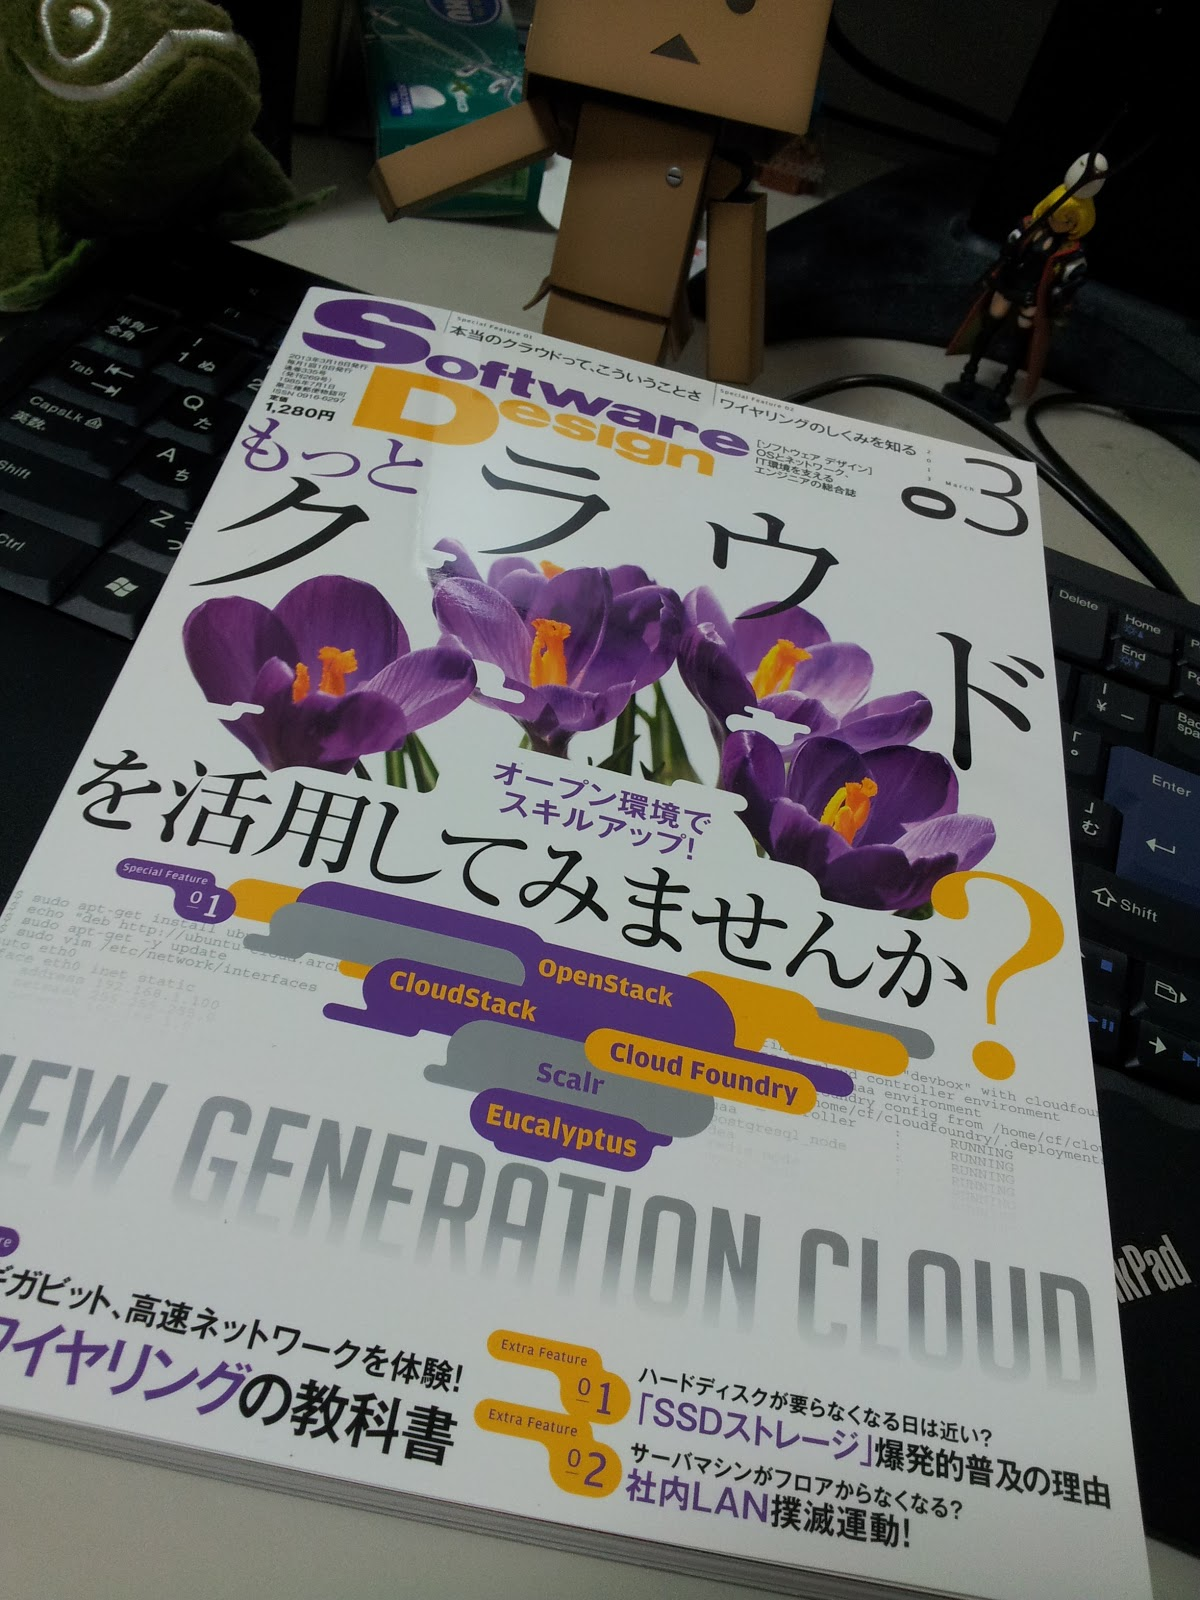
\includegraphics[height=0.5\textheight]{image201302/osc-tokyo/sd-201303-top.jpg}
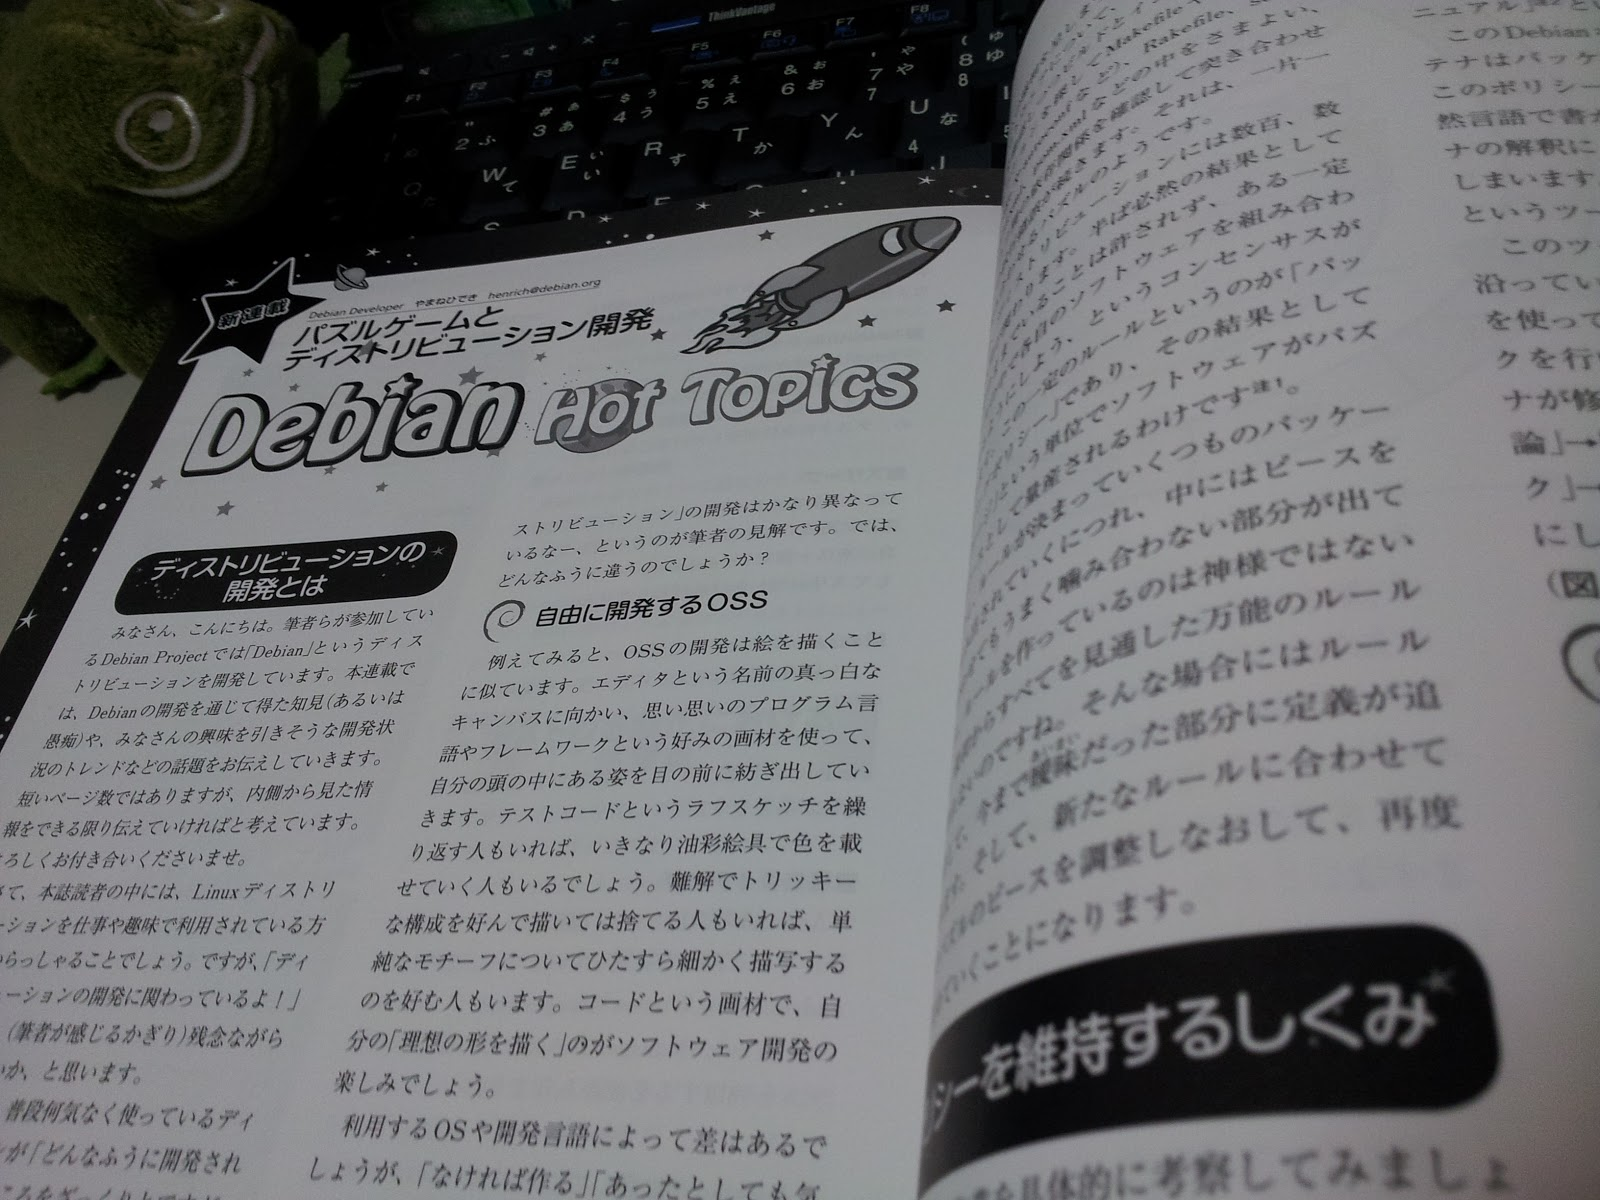
\includegraphics[height=0.5\textheight]{image201302/osc-tokyo/sd-201303-rensai.jpg}
\end{center}
\end{frame}
%画像はhenrichさんより提供
%http://henrich-on-debian.blogspot.jp/2013/02/debian-hot-topics.html

\begin{frame}
\begin{center}
\LARGE{Debian topic update}
\end{center}
\end{frame}

\begin{frame}{どこから喋る?}
\begin{center}
\Large{前回からのDebian topic updateについてお話すると、
なんと、2011年11月OSC Tokyo/Fallからになってしまいます...}
\end{center}
\end{frame}

\begin{frame}{どこから喋る?}
\Large
取り急ぎ、
\begin{itemize}
\item 古い話題については、大きなトピックのみを\\
(既にOSCにて発表済みは除く)
\item 新しい話題については、細かく
\end{itemize}
喋ります
\end{frame}

\begin{frame}{Lennyサポート終了}

\begin{center}
\LARGE{2012/2/6にてLennyのサポートが終了しました\\
みんな知ってるよね!?}
\end{center}
\url{http://www.debian.org/News/2012/20120209}
\end{frame}

\begin{frame}{Lenny→Squeezeへ}

\begin{center}
\LARGE{「え?まさか、まだアップグレードしてない!?」\\Squeezeへのアップグレードは↓}
\end{center}
i386版:
\url{http://www.debian.org/releases/stable/i386/release-notes/ch-upgrading.ja.html}や、\\
AMD64版:
\url{http://www.debian.org/releases/stable/amd64/release-notes/ch-upgrading.ja.html}等々
\end{frame}

\begin{frame}{ところでSqueeze update}

\begin{itemize}[<+->]
\item 2012/1/28 Debian 6.0.4 released \\
73個のセキュリティ修正と、87個のパッケージを更新。
(kernel側longtermリリースの変更点と、xenまわりの修正など)
\item 2012/5/12 Debian 6.0.5 released \\
74個のセキュリティ修正と、51個のパッケージを更新。
(kernel側longtermリリースの変更点など)
\item 2012/9/29 Debian 6.0.6 released \\
86個のセキュリティ修正と、52個のパッケージを更新。
(direct rendering manager(drm)のkernel側成果のマージ、閏秒対策など)
\end{itemize}

\end{frame}
% 6.0.4 \small{\url{http://www.debian.org/News/2012/20120128}}
% 6.0.5 \small{\url{http://www.debian.org/News/2012/20120512}}
% 6.0.6 \small{\url{http://www.debian.org/News/2012/20120929}}
% 変更点詳細:\small{\url{http://ftp.debian.org/debian/dists/sqeeze/ChangeLog}}

\begin{frame}
\begin{center}
\LARGE{パッケージ数}
\end{center}
\end{frame}

\begin{frame}{パッケージ数}
\begin{itemize}[<+->]

\item squeeze(stable)\\
バイナリパッケージ数: 28123 {\color{blue}-7}\\
ソースパッケージ数  : 14605 {\color{blue}-4}

\item whezzy(testing)\\ 
バイナリパッケージ数: 36167 {\color{red}+2893}\\
ソースパッケージ数  : 17332 {\color{red}+999}

\item sid(unstable)\\ 
バイナリパッケージ数: 38508 {\color{red}+3656}\\
ソースパッケージ数  : 18771 {\color{red}+1395}
\end{itemize}
\end{frame}

% squeezeパッケージ数は:
% \small{\url{http://ftp.debian.org/debian/dists/sqeeze/main/binary-amd64/Packages.gz}にてzegrep '^Package: 'して数える。なお、ちょうど7パッケージがsqueezeのChangeLogからリリース途中で廃止になったようなので、その分差っ引くと前回のOSC時の数とぴったり一致。}}
% squeezeソースパッケージ数は:
% \small{\url{http://ftp.debian.org/debian/dists/sqeeze/main/source/Sources.gz}にてzegrep '^Package: 'して数えた。}}
% Wheezyパッケージ数は:
% \small{\url{http://ftp.debian.org/debian/dists/wheezy/main/binary-amd64/Packages.gz}にてzegrep '^Package: 'して数えた。}}
% Wheezyソースパッケージ数は:
% \small{\url{http://ftp.debian.org/debian/dists/wheezy/main/source/Sources.gz}にてzegrep '^Package: 'して数えた。}}
% sidパッケージ数は:
% \small{\url{http://ftp.debian.org/debian/dists/sid/main/binary-amd64/Packages.gz}にてzegrep '^Package: 'して数えた。}}
% Wheezyソースパッケージ数は:
% \small{\url{http://ftp.debian.org/debian/dists/sid/main/source/Sources.gz}にてzegrep '^Package: 'して数えた。}}

\begin{frame}
\begin{center}
\LARGE{開発者数}
\end{center}
\end{frame}


\begin{frame}{開発者数}
\begin{itemize}[<+->]
\item 2011年11月\\
Debian Developer 約1470名 \\
Debian Maintainer 約80名

\item 2013年02月\\
Debian Developer 約1743名 \\
Debian Maintainer 約185名

\item 参考2012年6月時点で:59ヶ国\\
日本人  50名 (アクティブメンバ 35名)

\end{itemize}
\end{frame}
% ddの数は、\url{https://db.debian.org/}でカウント。
% 国別、アクティブ/非アクティブの情報は\url{http://www.perrier.eu.org/weblog/2012/06/06}のblog記事から
% DMの数は、\url{https://nm.debian.org/public/people}から、Debian Maintainerの数

\begin{frame}
\begin{center}
\LARGE{Debian カンファレンス}
\end{center}
\end{frame}

\begin{frame}{Debconf / Debian カンファレンス}
\begin{itemize}
\item 去年のDebconf, Debconf12 はニカラグア マナグアにて開催されました。\\
参加者は約180名。日本からは5名参加でした。
\item 今年のDebconf, Debconf13 はスイス ヴァーマルキュで開催となります。\\
2013年8月11日 から 18日 まで。\\
公式サイト:\url{http://debconf13.debconf.org}
\end{itemize}
\end{frame}

\begin{frame}{Debconf / Debian カンファレンス}
 去年のDebconf12では、Debian JP Projectのhenrichさんが、
Debian Packageの圧縮形式にxzを使うとDebianのアーカイブサイズを
大幅に圧縮できるよ!というテーマでBOFを開催されました。\\
BOFの様子:\url{http://www.youtube.com/watch?v=VwiPcgi8tIo}
\end{frame}

\begin{frame}{Debconf / Debian カンファレンス}
今年のDebconf13は、
\begin{itemize}
\item なんとスイスのキャンプ場で行われます。
\item 人里離れているキャンプ場なので、シェラフ持参のサバイバルな感じで行われるかも...
\end{itemize}
開催場所:\url{http://lecamp.ch/}\\
\begin{center}
\Large
!!奮ってのご参加の程お待ちしております!!
\end{center}
\end{frame}

\begin{frame}
\begin{center}
\LARGE{その他トピック}
\end{center}
\end{frame}

\begin{frame}{巷のWebサーバーOSの割合}
\begin{center}
\Large  w3techs.comの調査で2年連続 Webサーバーとして使われるディストリビューションの割合 No.1となった
\end{center}
\url{http://w3techs.com/blog/entry/debian_is_now_the_most_popular_linux_distribution_on_web_servers}
\url{http://w3techs.com/technologies/history_details/os-linux}
\end{frame}

\begin{frame}{巷のWebサーバーOSの割合}
\begin{center}
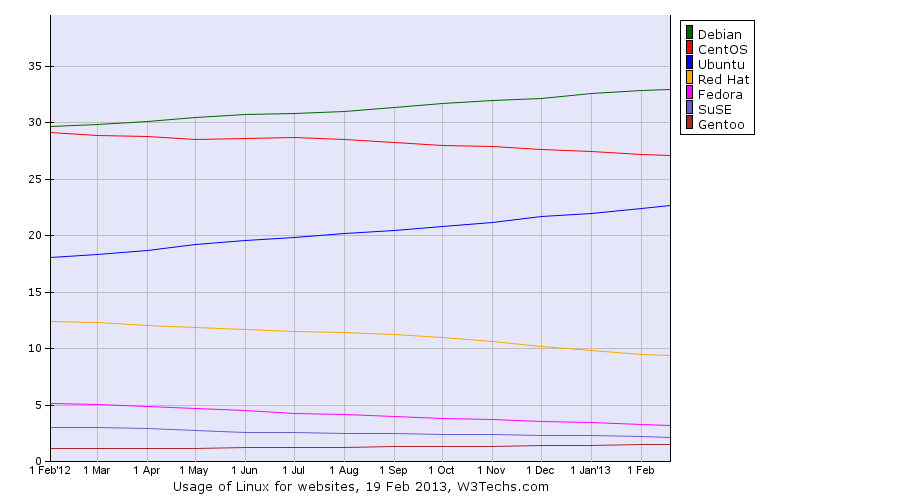
\includegraphics[width=1.0\hsize]{image201302/osc-tokyo/w3techs-graph.png}
\end{center}
\end{frame}
% グラフは
% http://w3techs.com/technologies/history_details/os-linux

\begin{frame}{遂にamd64が...}

2012/9/3のアナウンスによると、popconによる調査にて、
Debianのamd64アーキテクチャの利用率が、遂にi386を抜きました。

\begin{description}
\item [1位] amd64
\item [2位] i386
\item [3位] armel
\end{description}

\url{http://popcon.debian.org}

\end{frame}

\begin{frame}{日本国内の商標「DEBIAN\デビアン」が国際商標に統一}

 Debian JP Projectのmutoさんらの大変な尽力により、日本で所有していた
Debianの商標が無事SPIへ移管されました。これにより、国際商標
「DEBIAN」(国際登録番号:1084122)への統一・移行が完了しました。

この移行により、Debian の法的作業を担う団体による統一した形での運用となり、
Debianの商標への対応が迅速に可能となりました。

\url{http://www.spi-inc.org/corporate/resolutions/2012/2012-09-07.rtb.1/}\\
\url{https://lists.debian.org/debian-devel-announce/2012/10/msg00001.html}\\
\url{http://www.debian.or.jp/blog/debian_trademark_spi.html}
\end{frame}

\begin{frame}{日本国内の商標「DEBIAN\デビアン」が国際商標に統一}
\begin{center}
\Large
これまでの商標の維持、ならびに今回の移行にかかる費用をまかなう寄付を頂いた皆様方に深く感謝致します。
\end{center}
\end{frame}

\begin{frame}{debian-cloud開始(2012/12)}
cloud環境で利用できるDebianのイメージを開発するプロジェクト(debian-cloud)が
開始されました。
成果として、AWS Market Placeにて、Debian Squeezeのイメージが公開されています。\\
\url{http://deb.li/awsmp}\\
\url{http://wiki.debian.org/Cloud/AmazonEC2Image/Squeeze}\\
\url{http://aws.typepad.com/aws/2012/11/aws-marketplace-additional-operating-system-support.html}\\
プロジェクトのML:\\
\url{https://lists.debian.org/debian-cloud/}
\end{frame}

\begin{frame}{debian-cloud開始(2012/12)}

\begin{center}
\Large
Windows AzureにもDebianイメージが用意されました。\\
vmdepotでイメージを検索できます。
\end{center}
\end{frame}


\begin{frame}{debian-mobile開始(2012/12)}
いわゆるスマートフォンのような携帯端末でDebianを動かす為の
プロジェクトが開始されました。\\
\url{http://wiki.debian.org/Mobile}\\
\url{http://lists.debian.org/debian-mobile/}
\begin{center}
\Large ノートPCがなくなる前に携帯端末でDebianがネイティブブートで動くといいな!!\\(割と切実です)
\end{center}
\end{frame}


\begin{frame}{Debian 19歳}
\begin{center}

\Large{昨年2012年8月16日。Debian 19歳。}\\
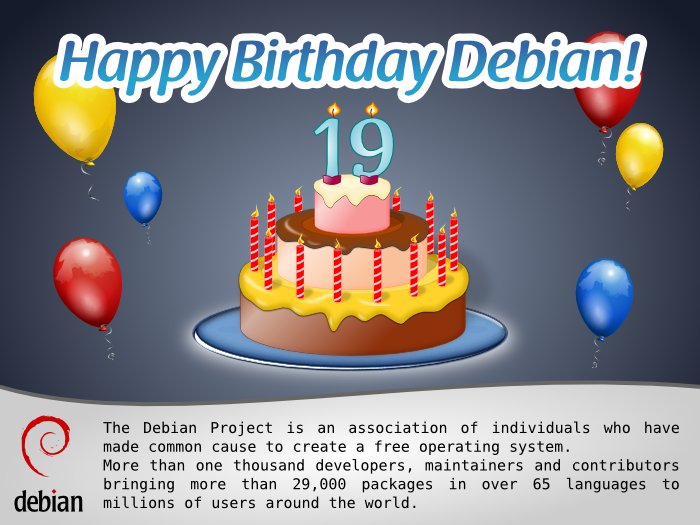
\includegraphics[width=0.8\hsize]{image201302/osc-tokyo/debian-19.png}
\end{center}
\Large{今年は20歳になる模様...}
\end{frame}
% debian-19.pngの画像は以下からダウンロード
% http://people.debian.org/~gismo/tmp/debian-19.png

\begin{frame}{Debian 19歳}

 Debianの誕生日である8/16周辺では、毎年お祝いということで、
各国でDebianDayが開かれます。\\
\url{http://wiki.debian.org/DebianDay} 

 当然日本もDebianDay 2012な事しました\\
\url{http://wiki.debian.org/DebianDay/2012\#DebianDay.2F2012.2FJapan.2FTokyo.Japan:_Tokyo}

\end{frame}

\begin{frame}{pbuilderのclang対応(2013/02)}

 巷ではCコンパイラとしてclangが流行っているわけですが、
当然Debianもこの流れに漏れずgccの他にclangを使ってみる試みがあります。\\
\begin{center}
\url{http://clang.debian.net/}
\end{center}
 で、debianパッケージのビルドテスト環境として、Debian JP Project所属の
上川さんによるpbuilderが有名なわけですが、こちらを先日clang対応の
パッチがhenrichさんにより作成され、bugs.debian.orgに投稿されました。\\
\url{http://bugs.debian.org/700290}
\begin{center}
\Large
パッケージに反映されると思うので、pbuilderがアップデートされたら\\
clangに興味ある方は、是非つかってみてくださいませー
\end{center}
\end{frame}

\begin{frame}{code search engine (2012/11)}

Debianソースパッケージのソースコードの検索サイトができたそうです。\\
\url{http://codesearch.debian.net/}

これは、
\begin{itemize}
\item 「そーいや、〜の関数を使っているパッケージってどれだっけ?」、
\item 「あの言語のあの関数/ライブラリの使い方はみんなどうしてるんだ?」
\end{itemize}
等の、開発関係者な悩みの日々をおくる皆様にぴったりなサービスです。

\end{frame}

\begin{frame}{増え続けるdebian mirrorサーバー}

 Debian使っていると、各国のmirrorサーバーにお世話になるわけですが、
mirrorサーバーをIPアドレスのおおよその地区情報(MaxMind社GeoLite)から起こして
世界地図に試しにプロットした人が現れました。\\
\begin{center}
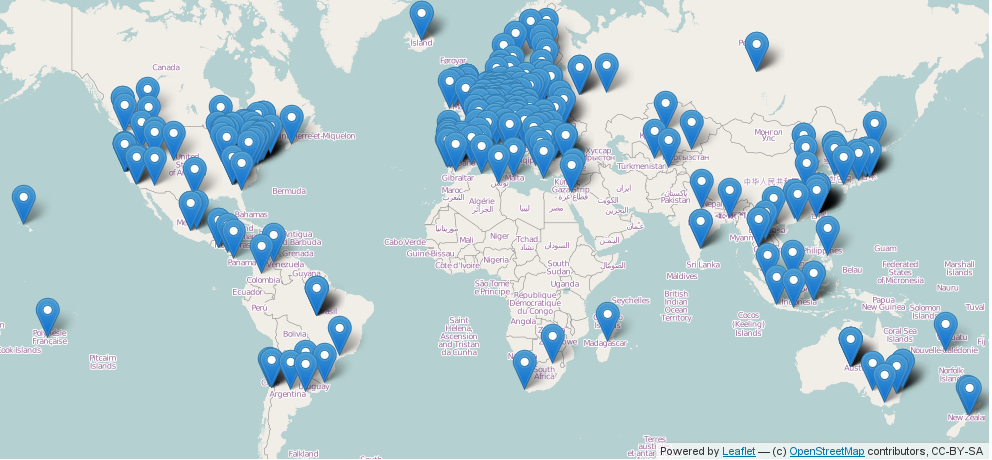
\includegraphics[width=0.8\hsize]{image201302/osc-tokyo/mirrors-map.png}
\end{center}
\url{http://rgeissert.blogspot.it/2012/10/debian-mirrors-map.html}\\
\begin{center}
まだまだ、いろいろな国に増えつづけていきます。
\end{center}
\end{frame}

\begin{frame}[containsverbatim]{http.debian.net}

 debianのmirrorサイトの負荷分散サイトとして、http.debian.netが出来ました。

\begin{commandline}
使い方の例: /etc/apt/sources.listにて、
# stableの場合
deb http://http.debian.net/debian stable main
\end{commandline}

 こちらは、redirect(HTTP 302)を利用したmirrorサーバーの負荷分散機構
となります。DNSベースの負荷分散サイトに比べてノードが落ちた時のDNS伝搬遅延などを
気にすることなく使えます。他の利点、情報については、\\
\url{http://http.debian.net/}
を参照ください。

\end{frame}

\begin{frame}{debian-mirror.sakura.ne.jp追加}

 さくらインターネット様にてご協力いただきまして、
Debianミラーサーバーがdebian-mirror.sakura.ne.jpとして
2/15より稼働開始しております。また、ftp.jp.debian.orgの
CDNミラーサーバーとしても追加済みです。

\begin{center}
\LARGE
ありがとうざいます、さくらインターネット様!
\end{center}

\end{frame}

\begin{frame}{cdimage.debian.or.jp 提供開始(2013/2/25追記)}

\Large
 株式会社アイティーシェルパ様(\url{http://itsherpa.com/})に
ご協力いただきまして、Debianの各cd/dvdイメージの日本国内配布サイト
の一つとして、
\begin{center}
\url{cdimage.debian.or.jp}
\end{center}
を追加しました。
\end{frame}

\begin{frame}{cdimage.debian.or.jp 提供開始(2013/2/25追記)}

ここで利用可能なイメージは、
\begin{itemize}
\item デスクトップLiveCD (GNOME)
\item デスクトップLiveCD (KDE)
\item デスクトップLiveCD (xfce4)
\item デスクトップLiveCD (LXDE)
\item amd64 (DVD / netinst)
\item i386 (CD / netinst)
\item kfreebsd-amd64
\item kfreebsd-i386
\end{itemize}
があります。\url{cdimage.debian.org}よりもダウンロード
速度の大幅改善が行われ、平均4倍以上が見込まれています。

\begin{center}
\LARGE
ありがとうざいます、アイティーシェルパ様!
\end{center}
\end{frame}

\begin{frame}
\begin{center}
\LARGE{Whezzyに向けての作業}
\end{center}
\end{frame}

\begin{frame}{現在の状況}
\huge{
\begin{itemize}
  \item \color{red}{2012/06/30 にフリーズ!! $\rightarrow$ 現在は}{\color{green}frozen}
  \item \color{red}{リリースに向けたバグ(RCバグ)潰しが進行中}
\end{itemize}
}
\end{frame}

\begin{frame}{現在の状況}

\begin{center}
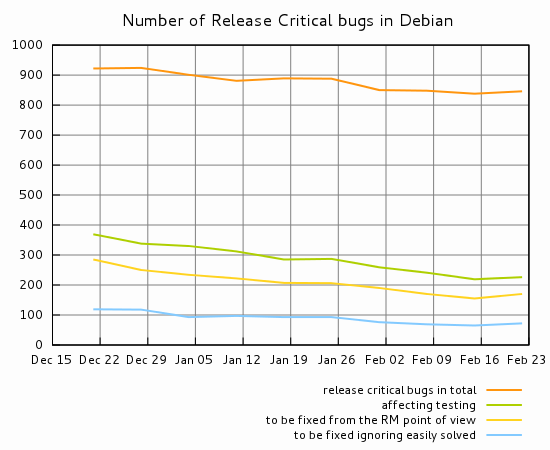
\includegraphics[height=0.7\textheight]{image201302/osc-tokyo/rc_bugs_report_en_2013-08.png}\\
\url{http://richardhartmann.de/blog/posts/2013/02/22-Debian_Release_Critical_Bug_report_for_Week_08/}
\end{center}

\end{frame}

\begin{frame}{WheezyのRCバグ}

\begin{center}
\LARGE
2/15現在、\\
194バグのうち、手つかずのバグが\color{red}{残り66バグ}\color{black}{のみです。}\\
Wheezyリリースに向けてバグ潰しをがんばりましょう!!
\end{center}

\end{frame}

\begin{frame}{参考:BSP in Japan!}

 パッケージのバグをみんなで集まって潰す集まりをBSP(Bug Squashing Party
バグ潰しパーティー)というのですが、henrichさん主催で、
OpenBlocksでお馴染みのぷらっとホーム様のご協力のもと、日本でも開かれました。\\

BSP 2012/11 jp Tokyo\\
 \url{http://wiki.debian.org/BSP/2012/11/jp/Tokyo}\\
開催のアナウンス\\
 \url{https://lists.debian.org/debian-devel-announce/2012/10/msg00009.html}

\end{frame}

\begin{frame}[containsverbatim]{multiarch}

 現在、Wheezyのリリースゴールのうち、multiarchについては完了。
そのため、ia32-libsパッケージ等は除去されました。\\
アナウンス: \url{https://lists.debian.org/debian-devel-announce/2013/01/msg00005.html}

 てっとり早くmultiarchの恩恵を味わうには、amd64環境のWheezy入れて
\begin{commandline}
apt-get install wine
\end{commandline}

をしてwineを実行してください。multiarchの設定を促されます。
\begin{center}
\Large
お試しあれ!
\end{center}
\end{frame}


\begin{frame}{インストーラ}
先日2013/02/17にて、Wheezyインストール用のインストーラリリース候補第1段の
Debian Installer 7.0 RC1がリリースされました。\\
※もちろん、Wheezyそのものではなく、インストーラプログラム本体ですよ。誤解なきよう。\\
アナウンス:\url{https://lists.debian.org/debian-devel-announce/2013/02/msg00005.html}\\
日本語アナウンス:\url{http://www.debian.or.jp/blog/wheezy_d-i_rc1.html}

\end{frame}

\begin{frame}{インストーラ}

 主な修正/変更点:
\begin{itemize}
\item アクセシビリティ機能への修正
\item kFreeBSDでの procfs マウントの修正
\item UEFIモードでの起動時のGRUBメニューの改善
\item 大量のドライバサポートの追加: 8021q, adm8211, at76c50x-usb, b43legacy, bnx2fc, cxgb4, cxgb4vf,fnic, igbvf, int51x1, isci, iwl4965, ixgbevf, libertas\_tf\_usb, micrel, mlx4\_en, mwifiex\_pcie, mwl8k, orinoco\_usb, pata\_piccolo, pch\_gbe, pmcraid, prism2\_usb, qlge, r8187se, r8192e\_pci, r8712u, rtl8192ce, rtl8192cu, rtl8192de, rtl8192se, smsc75xx, smsc9420, smsc95xx, tehuti, ums-eneub6250, ums-realtek, vt6656\_stage, vxge
\item 以下のRalink wifi のデバイス IDの追加: 5362, 5392, 539b
\item Lenovo 10/100 Ethernet USBドライバの追加
\end{itemize}
等など。詳しくは前ページのアナウンスを参照ください。

\end{frame}


\begin{frame}{リリースに向けてのご協力を!}
\begin{itemize}
 \item Debian を使ってください。
 \item 是非testing(Wheezy)にアップデートしましょう。
 \item BTSへバグ報告してください。些細なことでもなんでもOK。
 \item ドキュメント作成、翻訳に参加してください。\\
翻訳からTypoの指摘歓迎!
 \item パッケージメンテナンス等に興味がある方はサポートします。\\
そのへんにいる Debian 関係者に声をかけてください。
 \item 力のある方はバグ潰し歓迎!!
\end{itemize}
\end{frame}


\begin{frame}
\begin{center}
\LARGE{イベントのご紹介}
\end{center}
\end{frame}

\begin{frame}{東京エリア Debian勉強会}

\begin{center}
\Large
月1回土曜日関東でやってまーす
\end{center}

 Debian の開発者になれることをひそかに夢見るユーザたちと、 ある時にはそ
れを優しく手助けをし、またある時には厳しく叱咤激励する Debian 開発者ら
が Face to Face で Debian GNU/Linux のさまざまなトピック (新しいパッ
ケージ、Debian 特有の機能の仕組について、Debian 界隈で起こった出来事、
 etc ) について語り合います。

\end{frame}

\begin{frame}{東京エリア Debian勉強会}

 参加される方は主に東京を中心に関東近郊の国籍・性別不問の Debian ユー
ザです ( Debian をまだ使ったことが無いが興味があるので…とか、かなり遠
い所から来てくださる方もいます)。 開発の最前線にいる Debian の公式開発
者や開発者予備軍の方も居ますので、 普段は聞けないような様々な情報を得る
チャンスです。 興味と時間があった方、是非御参加下さい。 (また、勉強会
で話をしてみたいという方も随時募集しています。)

詳細は \url{http://tokyodebian.alioth.debian.org}をみてねー

\end{frame}

\begin{frame}{関西Debian勉強会}

\begin{itemize}
\item \url{http://wiki.debian.org/KansaiDebianMeeting}
\item  毎月第4日曜日. 13:30-17:00
\item 大阪(おもに福島区民センター)を中心に開催。たまに京都や奈良、神戸など
\end{itemize}

 関西 Debian 勉強会は関西の Debian Developer を増やすことを目標に 2007年から開催しています。関西エリアで Debian GNU/Linux のさまざまなトピック(新しいパッケージ、Debian 特有の機能や仕組み、Debian界隈で起こった出来事などなど)について話し合っており、来月 3 月の開催で 70 回目を迎えます。
\end{frame}

\begin{frame}{関西Debian勉強会}
 関西独自の企画としては、「月刊Debianポリシーマニュアル」という、毎月、一人がDebianポリシーマニュアルの章をまとめて発表する企画をしています。\\

 参加される方の中には、開発の最前線にいる Debian の公式開発者や開発者予備軍の方もいるので、普段聞けないような様々な情報を得るチャンスです。\\
\begin{center}
\Large
お時間が合えば、ぜひご参加下さい。
\end{center}
\end{frame}

\begin{frame}{その他イベント}

\begin{center}
\Large
 その他、いろいろなイベントを開いてます!!\\
詳しくは、\\
\url{http://www.debian.or.jp/}\\
みてねー。参加おまちしてまーす。
\end{center}

\end{frame}

\begin{frame}{その他イベント}
\begin{center}
\Huge
twitterでも情報発信中!\\
Twitter: @debianjp
\end{center}

\end{frame}

\begin{frame}{本日の展示}
\begin{center}
\Large
本日東京エリアDebian勉強会のブースだしてます。
\end{center}
展示物:
\begin{enumerate}
\item Wheezy PCの展示
\item あんどきゅめんてっどでびあんの展示/頒布
\item Debian のインフォグラフィック日本語版の配布
\item Debianステッカーの配布
\item Debian インストール CDの配布
\item 東京エリア/関西Debian勉強会の紹介
\end{enumerate}
\begin{center}
\Large
是非、お立ち寄りくださいませー
\end{center}

\end{frame}

\begin{frame}{質疑応答}
\begin{center}
\Large なにか質問はありますか?
\end{center}
\end{frame}



\end{document}

;;; Local Variables: ***
;;; outline-regexp: "\\([ 	]*\\\\\\(documentstyle\\|documentclass\\|emtext\\|section\\|begin{frame}\\)\\*?[ 	]*[[{]\\|[]+\\)" ***
;;; End: ***
